% The lexical route (Ch. 4).
\documentclass[12pt,border=2pt]{standalone}
\usepackage[T1]{fontenc}\usepackage{newtxtext}
\usepackage{tikz}\usetikzlibrary{positioning,arrows.meta,calc}
\begin{document}
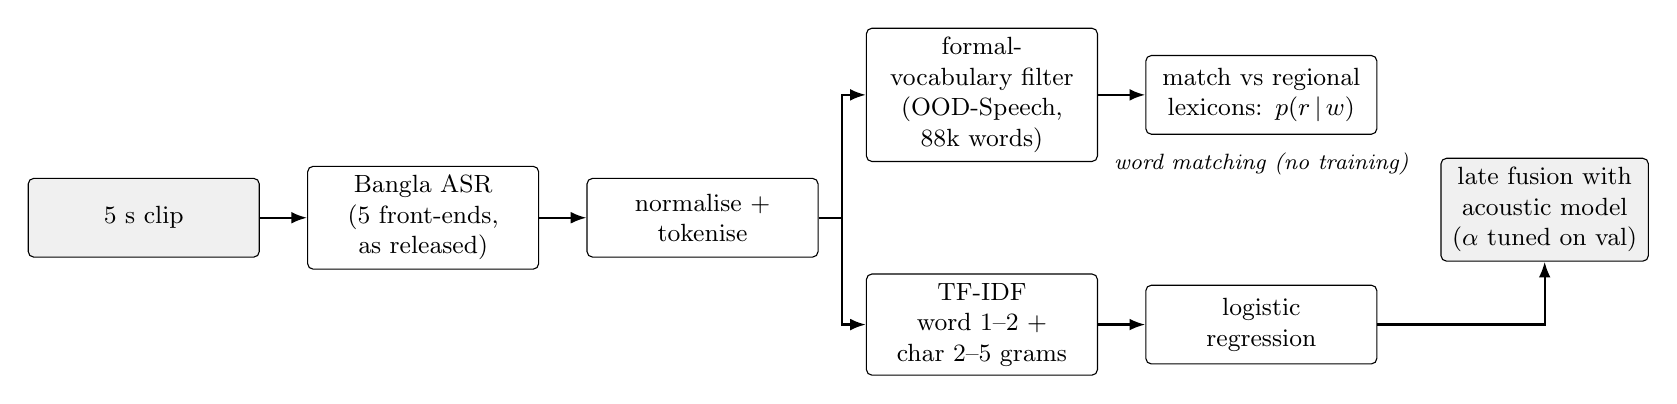
\begin{tikzpicture}[node distance=3mm and 6mm,
  box/.style={draw, rounded corners=2pt, align=center, font=\small, minimum height=10mm, text width=27mm, fill=white},
  data/.style={box, fill=black!6}, arr/.style={-{Latex[length=2mm]}, thick}]
  \node[data] (a) {5 s clip};
  \node[box, right=of a] (b) {Bangla ASR\\(5 front-ends,\\as released)};
  \node[box, right=of b] (c) {normalise +\\tokenise};
  \node[box, above right=2mm and 6mm of c] (d1) {formal-vocabulary filter\\(OOD-Speech, 88k words)};
  \node[box, below right=2mm and 6mm of c] (d2) {TF-IDF word 1--2 +\\char 2--5 grams};
  \node[box, right=of d1] (e1) {match vs regional\\lexicons: $p(r\,|\,w)$};
  \node[box, right=of d2] (e2) {logistic\\regression};
  \node[data, right=8mm of $(e1.east)!0.5!(e2.east)$, text width=24mm] (f) {late fusion with\\acoustic model\\($\alpha$ tuned on val)};
  \draw[arr] (a) -- (b); \draw[arr] (b) -- (c);
  \draw[arr] (c.east) -| ($(c.east)+(3mm,0)$) |- (d1.west); \draw[arr] (c.east) -| ($(c.east)+(3mm,0)$) |- (d2.west);
  \draw[arr] (d1) -- (e1); \draw[arr] (d2) -- (e2);
  \draw[arr] (e2.east) -| (f.south);
  \node[font=\footnotesize\itshape, below=1mm of e1] {word matching (no training)};
\end{tikzpicture}
\end{document}
